\documentclass[12pt,a4paper]{article}
\usepackage[utf8]{inputenc}
\usepackage[margin=2.5cm]{geometry}
\usepackage[slovene,english]{babel}
\usepackage[unicode]{hyperref}
\usepackage{
    lipsum,
    graphicx,
    amsmath,
    amssymb,
    caption,
    listings,
    color,
    subcaption,
    fancyhdr
}

\captionsetup[figure]{name=Graf}
\inputencoding{utf8}

\title{Primer statistične obdelave podatkov:\\ Telesna in možganska teža sesalcev}
\author{Erazem Kokot}
\date{2020}

\setcounter{tocdepth}{2}

\begin{document}

    \begin{titlepage}
        \maketitle

        \vfill
        \begin{center}
            Fakulteta za Računalništvo in Informatiko

            Verjetnost in Statistika
        \end{center}
        \thispagestyle{empty}
    \end{titlepage}
    
    \selectlanguage{slovene}

    \tableofcontents

    \renewcommand{\listtablename}{Kazalo tabel}
    \listoftables

    \renewcommand{\listfigurename}{Kazalo grafov}
    \listoffigures
    \thispagestyle{empty}

    \newpage

    \definecolor{mygreen}{rgb}{0,0.6,0}
\definecolor{mygray}{rgb}{0.5,0.5,0.5}
\definecolor{mymauve}{rgb}{0.58,0,0.82}

\lstset{ 
  backgroundcolor=\color{white},   % choose the background color; you must add \usepackage{color} or \usepackage{xcolor}; should come as last argument
  captionpos=b,                    % sets the caption-position to bottom
  commentstyle=\color{mygreen},    % comment style
  extendedchars=true,              % lets you use non-ASCII characters; for 8-bits encodings only, does not work with UTF-8
  firstnumber=1,                % start line enumeration with line 1000
  frame=single,	                   % adds a frame around the code
  keepspaces=true,                 % keeps spaces in text, useful for keeping indentation of code (possibly needs columns=flexible)
  keywordstyle=\color{blue},       % keyword style
  language=R,                 % the language of the code
  numbers=left,                    % where to put the line-numbers; possible values are (none, left, right)
  numbersep=7pt,                   % how far the line-numbers are from the code
  numberstyle=\tiny\color{mygray}, % the style that is used for the line-numbers
  rulecolor=\color{black},         % if not set, the frame-color may be changed on line-breaks within not-black text (e.g. comments (green here))
  showstringspaces=false,          % underline spaces within strings only
  stringstyle=\color{mymauve},     % string literal style
  tabsize=2,	                   % sets default tabsize to 2 spaces
}

    \section{Opis podatkov}


    \newpage
    \section{Opisna statistika}

Bonus točka V točki 2b) po Opisni statistiki, podajte razloge za transformacijo podatkov na
osnovi razsevnega diagrama, koeficienta korelacije in diagnostičnih grafov originalnih (netrans-
formiranih) podatkov. Potem pa nadaljujete z analizo v točkah 3-8.
    \newpage
    \section{Razsevni diagram in vzorčni koeficient korelacije}\label{sec3}

Prikažimo dobljene podatke na razsevnem diagramu:

\begin{figure}[h]
    \centering
    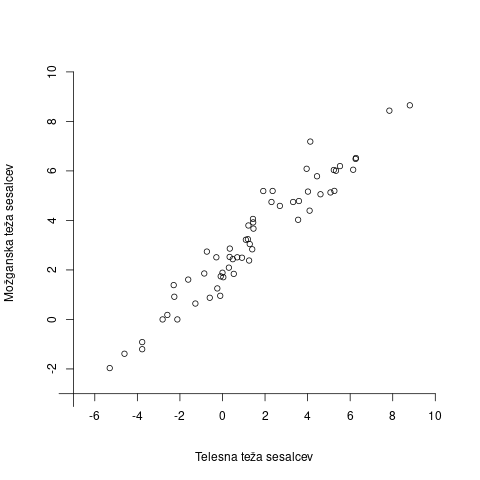
\includegraphics[scale=0.5]{res/razsevni-diagram.png}
    \caption{Razsevni diagram telesne in možganske teže sesalcev}
    \label{img:razs-diag}
\end{figure}

\noindent
Za izris grafa smo uporabili naslednjo R kodo:

\begin{verbatim}
    plot(
        x = log(mozgani$telteza),
        y = log(mozgani$mozteza),
        xlab = "Telesna teža sesalcev",
        ylab = "Možganska teža sesalcev",
        xlim = c(-7, 10),
        ylim = c(-3, 10),
        axes = FALSE
    )

    axis(1, pos = -3, at = seq(-8, 10, by = 2))
    axis(2, pos = -7, at = seq(-4, 10, by = 2))
\end{verbatim}

\newpage
Funkcija \verb|plot()| nam izriše razsevni diagram s podanimi parametri, v našem primeru z naslednjimi parametri:

\begin{itemize}
    \item \verb|x = log(mozgani$telteza)|, kjer \verb|x| predstavlja logaritemsko funkcijo telesne teže sesalcev,
    \item \verb|y = log(mozgani$mozteza)|, kjer \verb|y| predstavlja logaritemsko funkcijo možganske teže sesalcev,
    \item \verb|xlab| in \verb|ylab|, ki predstavljata ime x in y osi,
    \item \verb|xlim| in \verb|ylim|, ki določita začetne in končne koordinate x in y osi in
    \item \verb|axes = FALSE|, ki odstrani privzete koordinatne osi, saj jih želimo zamenjati z osmi, primernimi za
    naše parametre.
\end{itemize}

\noindent
Za izris koordinatnih osi uporabimo funkcijo \verb|axis()| s parametri \emph{1} ali \emph{2}, ki predstavljata
y in x os, \emph{pos}, ki predstavlja pozicijo postavitve osi, in \verb|at = seq()|, ki določi oznake na oseh
(s parametri \verb|seq(začetek, konec, razmak)|).
Moč korelacije lahko preverimo s \emph{Pearsonovim koeficientom}, kar v R naredimo z ukazom

\noindent
\verb|(r = cor(mozgani$telteza, mozgani$mozteza))|\label{en:r}, ki nam vrne rezultat \verb|[1] 0.9340911|.
Vrednost vzorčnega koeficienta korelacije je zelo visoka (r = 0.934), kar nakazuje visoko linearno povezanost
telesne teže sesalcev in teže njihovih možganov.
Ker je koeficient pozitiven nam to pove, da se z večjo telesno težo sesalca veča tudi teža njegovih možganov.
    \newpage
    \section{Formiranje linearnega regresijskega modela, prikaz računanja ocen naklona in odseka, ter enačba vzorčne regresijske premice}
    \newpage
    \section{Preverjanje predpostavk linearnega modela}
\subsection{Linearnost modela}
\subsection{Normalnost porazdelitve naključnih napak}
\subsection{Homogenost variance: graf in Breusch-Paganov test}
\subsection{Cookova razdalja: graf in analiza vpliva točk preko osnovnega pogoja, razsevnega diagrama in pogoja velikega vpliva}
    \newpage
    \section{Testiranje linearnosti modela in koeficient determinacije}

Poročilo o modelu lahko dobimo z ukazom \verb|summary(model)|, ki nam vrne spodnji (skrajšan) rezultat:

\begin{verbatim}
    Coefficients:
                Estimate Std. Error t value Pr(>|t|)    
    (Intercept)  2.17812    0.09487   22.96   <2e-16 ***
    lgtteza      0.74679    0.02773   26.93   <2e-16 ***
    ---
    Residual standard error: 0.6579 on 57 degrees of freedom
    Multiple R-squared:  0.9271,    Adjusted R-squared:  0.9259
    F-statistic: 725.4 on 1 and 57 DF,  p-value: < 2.2e-16
\end{verbatim}

Zanima nas samo testna statistika za testiranje linearnosti modela $T = 26.93$, z $df = 57$ prostorskimi
stopnjami, in p-vrednostjo $p = 2.2 \cdot 10^{16}$, ki je manjša od dane stopnje značilnosti 0.05.
S formalnim statističnim testiranjem smo potrdili, da linearni model ustreza podatkom.
Standardni odklon napak ocenjen s $S = 0.6579$, koeficient determinacije pa je enak $R^{2} = 0.9271$, kar je kvadrat
vzorčnega koeficienta korelacije. To pomeni, da 93\% variabilnosti telesne teže sesalcev pojasnjuje linearni regresijski
model.
    \newpage
    \section{Intervala zaupanja za naklon in odsek regresijske premice}

95\% interval zaupanja za neznani naklon in odsek regresijske premice lahko
izračunamo z ukazom \verb|round(confint(model), 3)|, ki nam vrne rezultat:

\begin{verbatim}
                2.5 % 97.5 %
    (Intercept) 1.988  2.368
    lgtteza     0.691  0.802
\end{verbatim}

Le-ta nam pove, da je interval zaupanja za odsek enak $I_{a} = [1.988, 2.368]$
in interval zaupanja za naklon enak $I_{b} = [0.691, 0.802]$.
    \newpage
    \section{Interval predikcije za vrednost Y pri izbrani vrednosti X}

Pri predvidevanju velikosti možganov sesalcev nas zanima bodoča vrednost spremenljivke Y (velikost možanov)
pri neki izbrani vrednosti spremenljivke X = $x_0$ (telesna teža).
Poleg predvidevane vrednosti $\widehat{y} = 95.8111 + 0.9653x_0$ za neke izbrane telesne teže sesalcev $x_0$ nas
zanimata tudi spodnja in zgornja meja, med katerima se nahaja velikost možganov sesalcev teh telesnih tež.
\emph{Interval predikcije} najdemo s pomočjo R funkcije \emph{predict()} in sicer z ukazoma
\verb|xteza = data.frame(telteza = c(100, 500, 2500))| in \verb|predict(model, xteza, interval = "predict")|,
ki nam vrne rezultate:

\begin{table}[h]
    \centering
    \begin{tabular}{cccc}
               & \textbf{fit} & \textbf{lwr} & \textbf{upr} \\
    \textbf{1} & 5.617202     & 4.277393     & 6.957011     \\
    \textbf{2} & 6.819109     & 5.464795     & 8.173424     \\
    \textbf{3} & 8.021017     & 6.646528     & 9.395506    
    \end{tabular}
    \caption{Interval predikcije}
    \label{tab:prediction}
\end{table}
    \newpage
    \section{Dodatno gradivo}

% Footer disclaimer
\pagestyle{fancy}
\fancyhf{}
\renewcommand{\headrulewidth}{0pt}
\cfoot{\emph{Zaradi limitacij LaTeX-a je koda prikazana brez šumnikov}}

\renewcommand{\lstlistingname}{Koda}
\lstinputlisting[caption=Generiranje slike razsevnega diagrama,label=code:mozgani]{res/razsevni-diagram.r}

\newpage
\lstinputlisting[caption=Formiranje linearnega regresijskega modela,label=code:model]{res/model.r}

\end{document}